\documentclass[Ligatures=TeX,table,brazil,svgnames,usetotalslideindicator,compress,10pt]{beamer}

\usetheme[titleformat=allsmallcaps]{metropolis}

\usepackage{polyglossia}
\setdefaultlanguage{brazil}
\disablehyphenation

\usepackage{minted}

\usetikzlibrary{arrows,positioning,calc}

\usepackage{graphicx}
\graphicspath{{./figuras/}}
\usepackage{subcaption}
\usepackage{xmpmulti}

% \usepackage{textpos}

% \usepackage{mdwlist}
% \usepackage{siunitx}
\usepackage{alltt}
% \usepackage{multicol}
\usepackage{xspace}
\usepackage{multirow}
\usepackage{amsmath}

\usepackage{cancel}

\newcommand{\setcoverbg}{
  \setbeamertemplate{background}
  {
\includegraphics[width=\paperwidth,height=\paperheight]{backgrounds/coverbg}}
}
\newcommand{\setintersectionbg}{
  \setbeamertemplate{background}
  {
\includegraphics[width=\paperwidth,height=\paperheight]{backgrounds/blank}}
}
\newcommand{\setsectionbg}{
  \setbeamertemplate{background}
  {
\includegraphics[width=\paperwidth,height=\paperheight]{backgrounds/slidebg2}}
}

\setbeamertemplate{caption}{default}

\title{MCTA025-13 - Sistemas Distribuídos}
\subtitle{Relógios Lógicos}

\author{Emilio Francesquini}
\institute{Centro de Matemática, Computação e Cognição\\ Universidade Federal do ABC}
\date{30 de julho de 2018}

\begin{document}

\setcoverbg
\maketitle

\setsectionbg

\begin{frame}
  \frametitle{Disclaimer}
  \begin{itemize}
  \item Estes slides foram preparados para o curso de \textbf{Sistemas
      Distribuídos na UFABC}.
  \item Este material pode ser usado livremente desde que sejam
    mantidos, além deste aviso, os créditos aos autores e
    instituições.
  \item Estes slides foram adaptados daqueles originalmente preparados
    (e gentilmente cedidos) pelo professor \textbf{Daniel Cordeiro, da
      EACH-USP} que por sua vez foram baseados naqueles
    disponibilizados online pelos autores do livro ``Distributed
    Systems'', 3ª Edição em:
    \url{https://www.distributed-systems.net}.
  \end{itemize}
\end{frame}


\setintersectionbg
\begin{frame}[standout]
    \begin{quotation}
      Num relógio é quatro e vinte,\\
      No outro é quatro e meia,\\
      É que de um relógio pro outro\\
      As horas vareia!
    \begin{flushright}
      \alert{Adoniran Barbosa}
    \end{flushright}
  \end{quotation}
\end{frame}
\setsectionbg

\begin{frame}
  \frametitle{Sincronização de relógios}
  \begin{itemize}
  \item relógios físicos
  \item relógios lógicos
  \item relógios vetoriais (Próxima Aula)
  \end{itemize}
\end{frame}

\begin{frame}
  \frametitle{Sincronização de Relógios}
  \begin{itemize}
  \item Em sistemas centralizados a definição do horário não é ambígua
  \item Em sistemas distribuídos isto não é verdade
    \begin{itemize}
    \item Mesmo em sistemas multi-processador pode não ser verdade
    \end{itemize}
  \end{itemize}

    \begin{block}{Exemplo de problema: Make}
    \begin{figure}
      \centering
      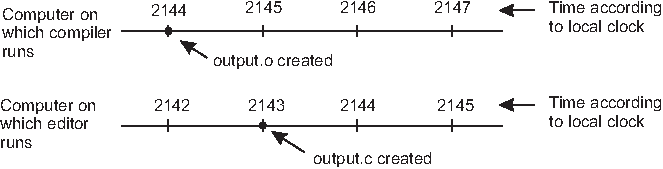
\includegraphics[width=.9\textwidth]{06-01}
    \end{figure}
  \end{block}

\end{frame}

\begin{frame}
  \frametitle{O que é um segundo?}
  \begin{itemize}
  \item \alert{Dia solar} - Tempo entre trânsitos solares
  \item \alert{Segundo solar} - Dia solar / 86400 (3600 * 24)
  \end{itemize}
  \begin{alertblock}{Problema}
    \begin{itemize}
    \item Em 1940 estabeleceu-se que o dia solar não é constante.
    \item Há 300 milhões de anos o ano tinha 400 dias.
    \end{itemize}
  \end{alertblock}
  O problema foi resolvido pegando a duração média do dia por um
  período muito longo.
\end{frame}

\begin{frame}
  \frametitle{Os relógios atômicos}
  \begin{itemize}
  \item Em 1948, com a invenção do relógio atômico passou a ser
    possível medir o tempo com muito mais precisão
  \item Os físicos então ``tomaram'' a definição do segundo dos astrônomos
    e definiram 1 segundo como o tempo que um átomo de césio 133 leva
    para fazer exatamente 9.192.631.770 transições
    \begin{itemize}
    \item Este era o valor exato do segundo solar na época da definição
    \item Deste então o segundo solar e O segundo divergiram em mais de 3 milissegundos
    \end{itemize}
  \end{itemize}
\end{frame}

\begin{frame}
  \frametitle{BIH e o TAI} Na metade do século passado foram
  instituídos o \textbf{Bureau International de l'Heure (BIH)} e o
  \textbf{Temps Atomique International (TAI)}.
  \begin{itemize}
  \item Todos os países poderiam, então, seguir o tempo seguindo o TAI
  \end{itemize}
  \begin{alertblock}{Problema}
    \begin{itemize}
    \item Como há uma defasagem entre o tempo solar e o tempo atômico
      em alguns milhares de anos o nascer do sol iria nascer ao meio dia
    \item Para corrigir essa defasagem estabeleceu-se o \alert{segundo bissexto}
      \begin{itemize}
      \item Introduzido sempre que a defasagem ultrapassar 800 milissegundos
      \end{itemize}
    \end{itemize}
  \end{alertblock}
\end{frame}

\begin{frame}
  \frametitle{Segundo bissexto}
    \begin{block}{Diferença entre UT1 e UTC}
    \begin{figure}
      \centering
      \vspace{-1em}
      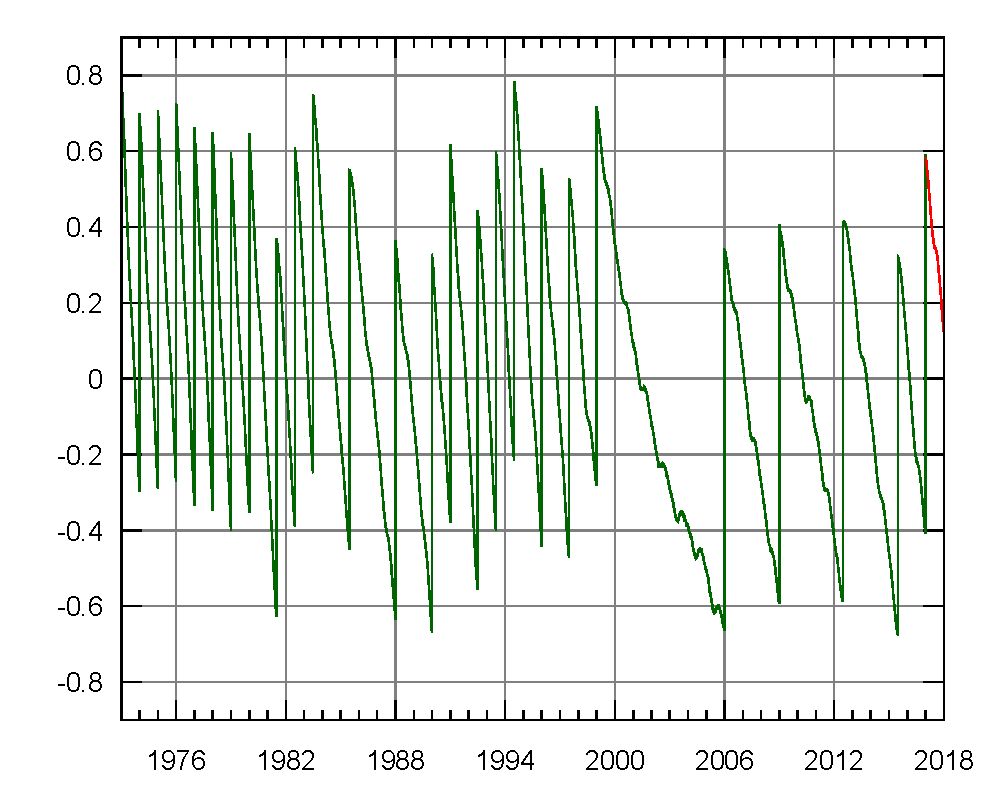
\includegraphics[width=.85\textwidth]{leap}
      \vspace{-1em}\caption{Wikipedia}
    \end{figure}
  \end{block}

\end{frame}


\begin{frame}
  \frametitle{Relógios Físicos}
  \begin{alertblock}{Problema}
    Algumas vezes precisamos saber a hora exata e não apenas uma ordenação de eventos.
  \end{alertblock}

  \begin{block}{Universal Coordinated Time (UTC):}
    \begin{itemize}
    \item baseado no número de transições por segundo do átomo de césio 133 (bastante preciso)
    \item atualmente, o tempo é medido como a média de cerca de 50 relógios de césio espalhados pelo mundo
    \item introduz um \emph{segundo bissexto} de tempos em tempos para compensar o fato de que os dias estão se tornando maiores
    \end{itemize}
  \end{block}
  \begin{block}{Nota:}
    O valor do UTC é enviado via \textit{broadcast} por satélite e por ondas curtas de rádio. Satélites tem um acurácia de ${\pm 0.5}$ ms.
  \end{block}
\end{frame}

\begin{frame}
  \frametitle{Curiosidade}
    Muitos relógios usam a frequência da rede elétrica (60Hz no
    Brasil) para manter a hora. Quando há segundos bissextos as
    companhias mantêm a frequência em 61 Hz por 60 segundos para
    adiantá-los.
\end{frame}

\begin{frame}
  \frametitle{Sincronização de relógios}

  \small

  \begin{block}{Precisão}
    O objetivo é tentar fazer com que o desvio \alert{entre dois relógios em quaisquer duas máquinas} fique dentro de um limite especificado, conhecido como a \alert{precisão} $\pi$:
    \[ \forall t, \forall p,q : | C_p(t) - C_q(t) | \le \pi \]
    onde $C_p(t)$ é o horário do relógio \alert{computado} para a máquina $p$ no \alert{horário UTC} $t$.
  \end{block}

  \begin{block}{Acurácia}
    No caso da \alert{acurácia}, queremos manter o relógio limitado a um valor $\alpha$:
    \[ \forall t, \forall p : | C_p(t) - t | \le \alpha  \]
  \end{block}

  \begin{block}{Sincronização}
    \begin{description}
    \item[Sincronização interna:] manter a \alert{precisão} dos relógios
    \item[Sincronização externa:] manter a \alert{acurácia} dos relógios
    \end{description}
  \end{block}
\end{frame}

\begin{frame}
  \frametitle{Flutuação dos relógios}
  \small
  \begin{block}{Especificação dos relógios}
    \begin{itemize}
    \item Todo relógio tem especificado sua \alert{taxa máxima de desvio do relógio} $\rho$.
    \item $F(t)$: frequência do oscilador do relógio do hardware no tempo $t$
    \item $F$: frequência (constante) do relógio ideal:
      \[ \forall t : (1-\rho) \le \frac{F(t)}{F} \le (1+\rho)  \]
    \end{itemize}
  \end{block}

  \begin{columns}[t]
    \begin{column}{.5\textwidth}
      \begin{block}{Observação}
        Interrupções de hardware acoplam um relógio de software a um relógio de hardware, que também tem sua taxa de desvio:
        \begin{align*}
          C_p(t) &= \frac{1}{F} \int^{t}_{0} F(t)dt \Rightarrow \frac{dC_p(t)}{dt} = \frac{F(t)}{F} \\
          &\Rightarrow \alert{\forall t: 1-\rho \le \frac{dC_p(t)}{dt} \le 1 + \rho}
        \end{align*}
      \end{block}
    \end{column}
    \begin{column}{.5\textwidth}
      \begin{block}{Relógios rápidos, perfeitos e lentos}
  \begin{figure}
    \centering
    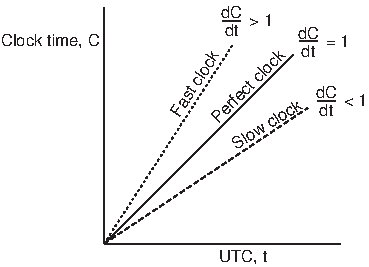
\includegraphics[width=.7\linewidth]{06-relogios}
  \end{figure}
        \end{block}
    \end{column}
  \end{columns}

\end{frame}

\begin{frame}
  \frametitle{Detectando e ajustando os horários}

  \begin{block}{Recuperação do horário atual de um servidor}
    \begin{figure}
      \centering
      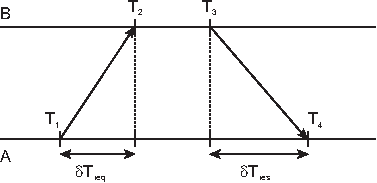
\includegraphics[width=.5\textwidth]{06-05}
    \end{figure}
  \end{block}
  \begin{block}{Cálculo da diferença relativa $\theta$ e o atraso $\delta$}
    \small
    Assumindo que: $\delta T_{req} = T_2 - T_1 \approx T_4 - T_3 = \delta T_{res}$
    \[
    \theta = T_3 + \bigl(( T_2 - T_1 ) + ( T_4 - T_3 )\bigr)/{2} - T_4 = \bigl(( T_2 - T_1 ) + ( T_3 - T_4 )\bigr)/{2}
    \]
    \[
    \delta = \bigl((T_4-T_1) - (T_3 -T_2)\bigr)/{2}
    \]
  \end{block}
  \begin{block}{Network Time Protocol}
    Colete oito pares ($\theta, \delta$) e escolha os $\theta$ cujos atrasos $\delta$ são minimais.
  \end{block}
\end{frame}

\begin{frame}
  \frametitle{Sincronização de relógios}

  \begin{block}{Sincronização externa}
    Cada máquina pede a um \emph{servidor de hora} a hora certa pelo menos uma vez a cada $\delta/(2\rho)$ (\alert{Network Time Protocol})
  \end{block}

  \begin{alertblock}{OK, mas...}
    você ainda precisa de uma maneira precisa de medir o \textit{round trip delay}, incluindo o tratamento da interrupção e o processamento das mensagens.
  \end{alertblock}

\end{frame}

\begin{frame}
  \frametitle{Sincronização de relógios}

  \begin{block}{Sincronização interna}
    Permita o servidor de hora sonde todas as máquinas periodicamente, calcule uma média e informe cada máquina como ela deve ajustar o seu horário \alert{relativo ao seu horário atual}.
  \end{block}

  \begin{alertblock}{Nota:}
    Você provavelmente terá todas as máquinas em sincronia. Você nem precisa propagar o horário UTC.
  \end{alertblock}

  \begin{alertblock}{É fundamental}
    saber que atrasar o relógio \alert{nunca} é permitido. Você deve fazer ajustes suaves.
  \end{alertblock}

\end{frame}


\setintersectionbg
\begin{frame}[standout]
    \begin{quotation}
      Relógio que atrasa não adianta.
    \begin{flushright}
      \alert{Desconhecido}
    \end{flushright}
  \end{quotation}
\end{frame}
\setsectionbg

\section{Relógios lógicos}

\begin{frame}
  \frametitle{Problema}
  \begin{alertblock}{}
    O que importa na maior parte dos sistemas distribuídos não é fazer
    com que todos os processos concordem exatamente com o horário, mas
    sim fazer com que eles concordem com \alert{a ordem em que os
      eventos ocorreram}. Ou seja, precisamos de uma noção de ordem
    entre os eventos.
  \end{alertblock}
\end{frame}

\begin{frame}
  \frametitle{A relação ``aconteceu-antes''}

  \begin{block}{A relação ``aconteceu-antes'' (\textit{happened-before})}
    \begin{itemize}[<+->]
    \item se $a$ e $b$ são dois eventos de um mesmo processo e $a$ ocorreu antes de $b$, então $a \rightarrow b$
    \item se $a$ for o evento de envio de uma mensagem e $b$ for o evento de recebimento desta mesma mensagem, então $a \rightarrow b$
    \item se $a \rightarrow b$ e $b \rightarrow c$, então $a \rightarrow c$
    \end{itemize}
  \end{block}
  \pause
  \begin{block}{Eventos concorrentes}
  Se dois eventos $x$ e $y$ ocorrem em processos distintos e
  esses processos nunca interagem (mesmo que indiretamente) então nem
  $x \rightarrow y$ nem $y \rightarrow x$ são verdade. São
  eventos \alert{concorrentes}. Quando se diz que dois eventos são
  concorrentes na verdade quer dizer que \emph{nada pode (ou precisa) ser
    dito sobre a sua ordem}.
  \end{block}
  \pause
  \begin{alertblock}{Nota:}
    Isso introduz uma noção de \alert{ordem parcial dos eventos} em um sistema com processos executando concorrentemente.
  \end{alertblock}

\end{frame}


\begin{frame}
  \frametitle{Relógio lógico de Lamport}
  \begin{alertblock}{Problema}
    Como fazemos para manter uma visão global do comportamento do sistema que seja consistente com a relação aconteceu-antes?
  \end{alertblock}

  \pause
  \begin{block}{Solução}
    Associar um \textit{timestamp} $C(e)$ a cada evento $e$ tal que:
    \begin{description}
    \item[P1] se $a$ e $b$ são dois eventos no mesmo processo e $a \rightarrow b$, então é obrigatório que $C(a) < C(b)$
    \item[P2] se $a$ corresponder ao envio de uma mensagem $m$ e $b$ ao recebimento desta mensagem, então também é válido que $C(a) < C(b)$
    \end{description}
  \end{block}

  \pause
  \begin{alertblock}{Outro problema}
    Como associar um \textit{timestamp} a um evento quando não há um relógio global? Solução: manter um conjunto de relógios lógicos \alert{consistentes}, um para cada processo
  \end{alertblock}

\end{frame}

\begin{frame}
  \frametitle{Relógio lógico de Lamport}

  \begin{block}{Solução}
    Cada processo $P_i$ mantém um contador $C_i$ \alert{local} e o ajusta de acordo com as seguintes regras:
    \begin{enumerate}
    \item para quaisquer dois \textbf{eventos sucessivos} que ocorrer em $P_i$, $C_i$ é incrementado em 1
    \item toda vez que uma mensagem $m$ for \alert{enviada} por um processo $P_i$, a mensagem deve receber um \textit{timestamp} $ts(m) = C_i$
    \item sempre que uma mensagem $m$ for \alert{recebida} por um processo $P_j$, $P_j$ ajustará seu contador local $C_j$ para \alert{$\max\{C_j, ts(m)\}$} e executará o passo 1 antes de repassar $m$ para a aplicação
    \end{enumerate}
  \end{block}

  \begin{block}{Observações:}
    \begin{itemize}
    \item a propriedade \textbf{P1} é satisfeita por (1); propriedade \textbf{P2} por (2) e (3)
    \item ainda assim pode acontecer de dois eventos ocorrerem ao mesmo tempo. \alert{Desempate usando os IDs dos processos}.
    \end{itemize}
  \end{block}

\end{frame}

\begin{frame}
  \frametitle{Relógio lógico de Lamport -- exemplo}

  Considere três processos com \alert{contadores de eventos} funcionando a velocidades diferentes.

  \begin{figure}
    \centering
    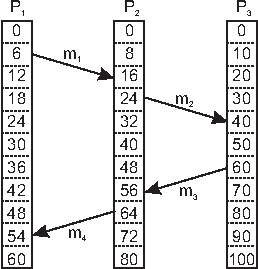
\includegraphics{06-08a}
    \hfill{}
    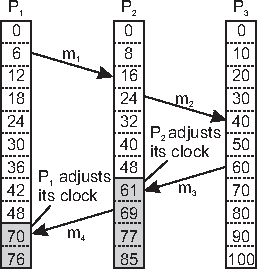
\includegraphics{06-08b}
  \end{figure}

\end{frame}

\begin{frame}
  \frametitle{Relógio lógico de Lamport -- exemplo}

  \begin{alertblock}{Nota}
    Os ajustes ocorrem na camada do \textit{middleware}
  \end{alertblock}

  \begin{figure}
    \centering
    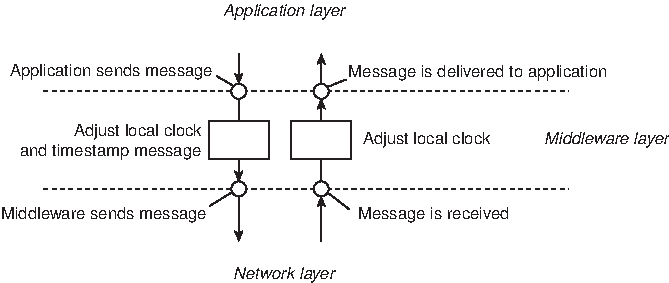
\includegraphics{06-10}
  \end{figure}

\end{frame}

\begin{frame}
  \frametitle{Exemplo: multicast com ordem total}
  \begin{alertblock}{Problema}
    Alguma vezes precisamos garantir que atualizações concorrentes em um banco de dados replicado sejam vistos por todos como se tivessem ocorrido na mesma ordem.

  \begin{itemize}
  \item $P_1$ adiciona R\$ 100 a uma conta (valor inicial: R\$ 1000)
  \item $P_2$ incrementa a conta em 1\%
  \item Há duas réplicas
  \end{itemize}
\end{alertblock}

\begin{figure}
  \centering
  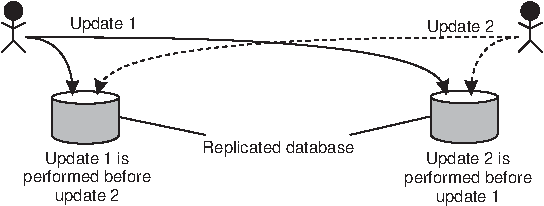
\includegraphics[scale=0.6]{06-11}
\end{figure}

\vspace{-1ex}
\begin{block}{Resultado}
  Na ausência de sincronização correta, \newline réplica \#1 $\leftarrow$ R\$ 1111, enquanto que na réplica \#2 $\leftarrow$ R\$ 1110.
\end{block}

\end{frame}

\begin{frame}
  \frametitle{Exemplo: multicast com ordem total}

  \begin{block}{Solução}

    \begin{itemize}
    \item processo $P_i$ envia uma \alert{mensagem com timestamp} $m_i$ para todos os outros. A mensagem é colocada em sua fila local $queue_i$.
    \item toda mensagem que chegar em $P_j$ é colocada na fila $queue_j$ \alert{priorizada pelo seu timestamp} e \alert{confirmada} (\textit{acknowledged}) por todos os outros processos
    \end{itemize}
  \end{block}

  \framebox{%
    \begin{minipage}{0.97\textwidth}
      \textbf{$P_j$ repassa a mensagem $m_i$ para a sua aplicação somente se:}
      \begin{enumerate}
      \item[(1)] $m_i$ estiver na cabeça da fila $queue_j$
      \item[(2)] para todo processo $P_k$, existe uma mensagem $m_k$ na $queue_j$ com um \textit{timestamp} maior.
      \end{enumerate}
  \end{minipage}}

\begin{alertblock}{Nota}
  Assumimos que a comunicação é \alert{confiável} e que a \alert{ordem FIFO} (entre as mensagens enviadas por um nó, e não na fila)  é respeitada.
\end{alertblock}

\end{frame}

\begin{frame}
  \frametitle{O algoritmo de multicast funciona?}
  % https://cis.temple.edu/~giorgio/cis307/readings/newlogicalClock.html
  % Does this algorithm work? Let's first observe that when a message
  % m becomes ready at a site S, m has been received by all the sites
  % since they have given an acknowledgement for m that was received
  % at S. Second, if n is a message originated from the same site as m
  % and sent before m, then everywhere n is received before m and the
  % acknowledgements for n are received everywhere before the
  % acknowledgements for m (this is so because of the properties
  % assumed for links) thus n will be be ready before m and will be
  % delivered to the application (be extracted from the queue) before
  % m. So for each message originating site we need to worry only
  % about one message from that site (the other messages from that
  % site will be naturally delayed relative to the first one) If
  % message n originates from a different site than m the argument is
  % harder to make. It is possible that m and n are delivered in
  % different order at different sites. But it is certain that before
  % making the final decision to remove from queue either m or n, that
  % both m and n and one acknowledgement of either m or n will be
  % received at each site thus allowing the algorithm to compare
  % clocks and possibly delay dequeueing in order to respect the clock
  % total order. That is, in all cases, if n precedes m in the total
  % order then n will become ready before m. Thus messages are
  % delivered to the application in their clock order. The following
  % diagram illustrates the situation. Machine M2 sends message m and
  % machine M3 sends message n. To simplify the diagram we show only
  % the messages delivered to M1 and M4. The acknowledgements are
  % indicated with a broken line and a primed name.

  Observe que:
  \begin{itemize}
  \item se uma mensagem $m$ ficar pronta em um servidor $S$, $m$ foi
    recebido por todos os outros servidores (que enviaram ACKs dizendo
    que $m$ foi recebido)
  \item se $n$ é uma mensagem originada no mesmo lugar que $m$ e for
    enviada antes de $m$, então todos receberão $n$ antes de $m$ e $n$
    ficará no topo da fila antes de $m$
  \item se $n$ for originada em outro lugar, é um pouco mais
    complicado. Pode ser que $m$ e $n$ cheguem em ordem diferente nos
    servidores, mas é certeza de que antes de tirar um deles da fila,
    ele terá que receber os ACKs de todos os outros servidores, o que
    permitirá comparar os valores dos relógios e entregar para as
    mensagens na ordem total dos relógios
  \end{itemize}

\end{frame}

% \begin{frame}[fragile]
%   \frametitle{Relógio de Lamport para exclusão mútua}
%   \tiny
% \begin{minted}{python}
% class Process:
%   def __init__(self, chan):
%     self.queue      = []                     # The request queue
%     self.clock      = 0                      # The current logical clock

%   def requestToEnter(self):
%     self.clock = self.clock + 1                         # Increment clock value
%     self.queue.append((self.clock, self.procID, ENTER)) # Append request to q
%     self.cleanupQ()                                     # Sort the queue
%     self.chan.sendTo(self.otherProcs, (self.clock,self.procID,ENTER)) # Send request

%   def allowToEnter(self, requester):
%     self.clock = self.clock + 1                         # Increment clock value
%     self.chan.sendTo([requester], (self.clock,self.procID,ALLOW)) # Permit other

%   def release(self):
%     tmp = [r for r in self.queue[1:] if r[2] == ENTER]  # Remove all ALLOWs
%     self.queue = tmp                                    # and copy to new queue
%     self.clock = self.clock + 1                         # Increment clock value
%     self.chan.sendTo(self.otherProcs, (self.clock,self.procID,RELEASE)) # Release

%   def allowedToEnter(self):
%     commProcs = set([req[1] for req in self.queue[1:]]) # See who has sent a message
%     return (self.queue[0][1]==self.procID and len(self.otherProcs)==len(commProcs))
% \end{minted}
% \end{frame}

% \begin{frame}[fragile]
%   \frametitle{Relógio de Lamport para exclusão mútua}
%   \scriptsize
% \begin{minted}{python}
%   def receive(self):
%     msg = self.chan.recvFrom(self.otherProcs)[1]  # Pick up any message
%     self.clock = max(self.clock, msg[0])          # Adjust clock value...
%     self.clock = self.clock + 1                   # ...and increment
%     if msg[2] == ENTER:
%       self.queue.append(msg)                      # Append an ENTER request
%       self.allowToEnter(msg[1])                   # and unconditionally allow
%     elif msg[2] == ALLOW:
%       self.queue.append(msg)                      # Append an ALLOW
%     elif msg[2] == RELEASE:
%       del(self.queue[0])                          # Just remove first message
%     self.cleanupQ()                               # And sort and cleanup
% \end{minted}
% \end{frame}

% \begin{frame}
%   \frametitle{Relógio de Lamport para exclusão mútua}
%   \begin{block}{Analogia com multicast de ordem total}
%     \begin{itemize}
%     \item No multicast de ordem total, todos os processos construíam
%       fila idênticas, entregando as mensagens na mesma ordem
%     \item Exclusão mútua implica em concordar sobre a ordem em que os
%       processos devem ter sua entrada permitida na seção crítica
%     \end{itemize}
%   \end{block}
% \end{frame}


\end{document}
